\section{Implementation} 
\label{sec:implementation}

We now present \prodscalpel, our realisation of \FOUNDRY for C. \prodscalpel extends $\mu$Scalpel~\cite{Barr2015} to transplant multiple organs at once and implant them into a single host codebase. This feature is essential for supporting \FOUNDRY, since many features, especially those existing, SPL-oblivious codebases, span multiple files.

%\eb{from leandro: I've write these two next sentences describing the figure 7 while it makes a connection between section 3 and 4.}

The overall architecture of \prodscalpel comprises five distinct modules, as depicted in Figure \ref{fig:prodscalpel}. These modules serve as integral components of the \prodscalpel solution, implementing the different stages of \FOUNDRY for the reengineering of systems into SPL. 
The domain engineering process is automated by the \textit{Preprocessing and cleansing} and the \textit{Over-organ extraction} modules. The first one is responsible for cleansing the donor codebases, eliminating any extraneous preprocessor directives that may be present. It also used to host preparing process by removing undesired features delimited by preprocessor directives from the product base. On the other hand, the \textit{Over-organ extraction} module employs the program slicing technique implemented with SGD to extract an over-organ from the donor codebase, thereby isolating the relevant code fragments for further adaptation.

%This step ensures that the host codebase is streamlined for the subsequent transplantation process.

The application engineering process is automated by the \textit{Over-organ reduction and adaptation}, and the \textit{Organ implantation} modules. The first one utilizes genetic programming (GP) to reduce the size and complexity of the selected over-organ obtained from the transplantation platform. This reduction process is carried out while ensuring that the over-organ is effectively adapted to function within the target product base. GP enables the systematic exploration and optimization of the organ's code structure, achieving an organ specialized to a specific product base. The \textit{Organ implantation}, in turn, employs a clone detector to identify code elements duplication and dependencies during the process of implanting the organ into the product base.

More details on how \prodscalpel automates the \FOUNDRY process is provided in the following sections.

\begin{figure*}[t]
	\centering  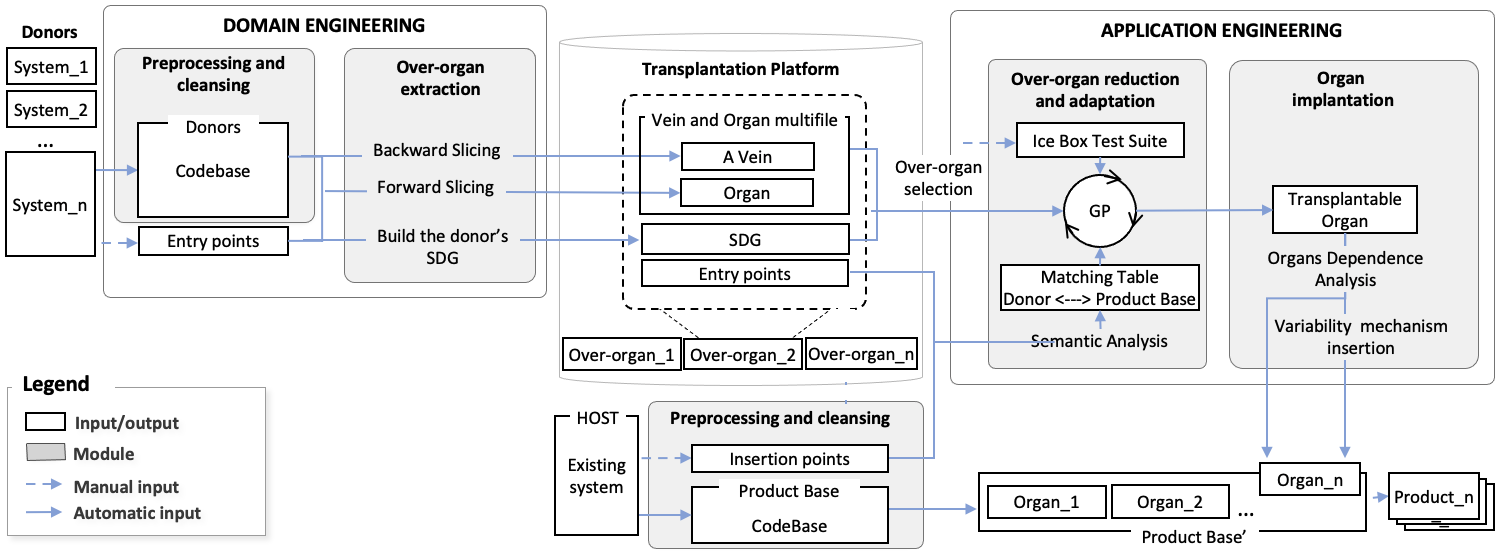
\includegraphics[width=\textwidth]{images/PRODSCALPEL_ARCHITECTURE.png}
	\centering \caption{Overall architecture of \prodscalpel. \textit{An SDG is a system dependency graph that the genetic programming phase uses to constrain its search space.}
 }
	\label{fig:prodscalpel}
\end{figure*} 

\subsection{Automating Feature Removal}

First we need to select and prepare our product base. The selected program might contain some unwanted features for the target product, thus we want to remove them before transplantation takes place. To automate removing unwanted features and dead code from the donor and host systems, \prodscalpel  implements a  \emph{Reconfigurator}. To work, \prodscalpel initially requires engineers to provide as input a textual list of preprocessor directives corresponding to each feature and annotation to be removed. From this, the tool searches for pieces of code that implement features limited by preprocessor directives, removing them from the product base. \prodscalpel then maps and searches selectively for pieces of code that implement features limited by such directives. Then, \prodscalpel removes all features source code from the product base while it keeps the source code structure belonging to the product base unchanged and ready to receive the transplanted organs. \Cref{fig:reconfigurator} gives a example of a portion of code after \prodscalpel cleaned up unused directives. 

\begin{figure}[t]
	\centering 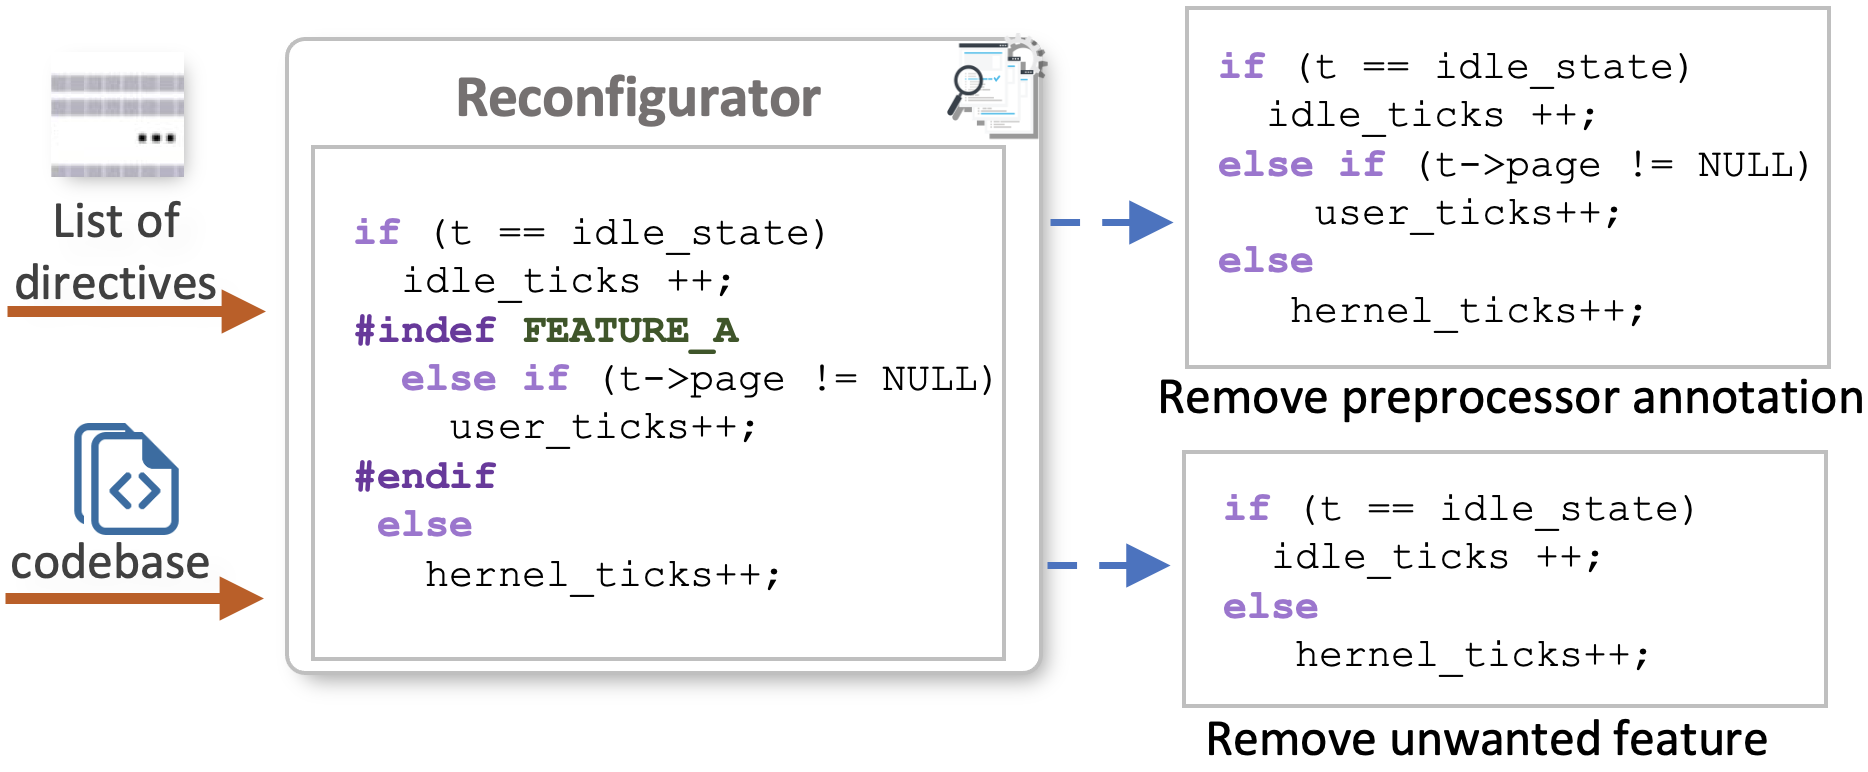
\includegraphics[width=0.7\textwidth]{images/reconfigurator2.png}
	\centering 
	\caption{The reconfigurator used to automated removal of preprocessor annotation from donor codebase and unwanted features from product base.}
	\label{fig:reconfigurator}
\end{figure} 

\subsection{Automating Vein and Over-Organ Extraction}
As optimisations, \prodscalpel extracts the vein from multiple files. \prodscalpel uses backward slicing to identity each function belonging to the vein and saves it in a copy of its souce file in the transplantation platform. Then, it includes all functions calling existing into vein source code in the \emph{array of over-organ statements} used by GP to achieve an organ from the over-organ~\cite{Barr2015}. Thus,  a function/method in the vein shared between two organs is not duplicated when transplanted.

\prodscalpel avoids the problem of vein redundancy when a great part of the vein is common for multiple organs transplanted from the same donors. The vein duplication is discovered by the implantation module during the implantation stage. In the extraction stage, both veins belonging to two organs (A and B) are kept duplicated in the transplantation platform in different directories, since it is important to keep the over-organ functional. However, when the second organ( organ B) is implanted after the transplant of organ A, the code clone detector looks for duplication also in the vein code of organ A. For example, imagine that a vein has a function $\texttt{fx()}$ implemented in file $\texttt{F\.c}$ and belonging to both over-organs A and B. When \prodscalpel tries to transplant organ B after organ A, it checks if the function  $\texttt{fx()}$ already exists in file F.c in the post-operative environment. In this way, if the function  $\texttt{fx()}$ is already in the host post-operative, as part of organ A, \prodscalpel does not insert it into the host again. Instead, the function $\texttt{fx()}$ already transplanted also is used by organ B.

\prodscalpel also identifies occurrences of mutually recursive functions, even an occurrence of an indirect recursion. Technically, \prodscalpel inlines the vein code while puts each function found in a stack of functions. When \prodscalpel finds an occurrence of a recursive function it recovers the beginning of the recursive call and does not inline it. Instead, \prodscalpel extracts the function to a file with the same name of the where the function is implemented. Then, it inserts a calling from the vein to the recursive function. This solution provides a finite interpretation for not inlining mutually recursive functions in the array of over-organ statements. Thus, \prodscalpel can produce a search space for GP with a finite amount of program statements even from recursive functions.

To handle transplantation of organs spread in multiple files, \prodscalpel records the name of the files where the slice is and its location with respect to other slices from the over-organ. 
Then, it records the related statements in an Abstract Syntax Tree (AST), according to their order of appearance in the file. 
This is done to preserve the same structure in the transplanted organ as it appeared in the donor.
Then, \prodscalpel computes the resulting slices in copies of its original files  in the transplantation platform, without breaking the over-organ.


\subsection{Automating Over-organ Reduction and Adaptation}\label{sec:organ_reduction}
\prodscalpel improves the process of over-organ reduction and adaptation by being able to handle over-organs containing multiple files.
It also introduces a layer in the organ that works as an organ-host wrapper. 

In practice, \prodscalpel uses GP, as in previous work~\cite{Barr2015}, to prune one or more program elements within the boundaries of the target organ while keeping the organ still functional and passing on the icebox tests. 
In the wrapper, \prodscalpel~abstracts variable names so that GP can select a type-compatible binding. It selects different combinations of all valid statements, variables and function calls mapped from the organ's vein to initialise an execution environment that the organ expects before executing it. 

\prodscalpel uses GP to search for matching between variables in the organ and the product base, during the over-organ adaptation process. The matches found are inserted in the organ-host wrapper. 
By a mutation operation, a new version of the organ (i.e., a new individual) is created while \prodscalpel makes several changes in the organ-host wrapper and pruning the over-organ. Each such mutation operation is either an $\texttt{INSERT}$, $\texttt{REPLACE}$ and $\texttt{DELETE}$ of code into the individual and the wrapper at the level of statements.

In the end, \prodscalpel synthesises a call to the extracted organ to execute and test it from the wrapper constructed.

\subsection{Automating Multiple Organ Implantation}
\label{sec:Implantation}


Once the organ is adapted to correctly work on the host it can be automatically implanted into the product base. To correctly insert an organ into the tool must identify and handle potential implicit connection points by avoiding the insertion of code duplication into the product base.

\Cref{fig:code_clone_analysis} illustrates our solution to avoid the organ collision problem. To sum up, the clone detector checks if a specific code element is already present in the beneficiary's environment. To do this, \prodscalpel constructs two lists, one with elements in the organ and other with elements in the host. Then, it checks if there is some element in the target organ which is already presented in a list of code elements transplanted. Once a potential element duplication is identified, \prodscalpel decomposes both organ and host elements in ASTs to detect semantic dependencies between organ implementations previously transplanted, preventing shared elements to be inserted into the host again. Then, the code element is entirely \emph{grafted}, \emph{discarded}, or \emph{merged}. In this last case, \prodscalpel introduces additional line breaks such that potential variances within statements and other structures can be accurately inserted by using sub-abstract tree comparison.

\begin{figure}[t]
	\centering 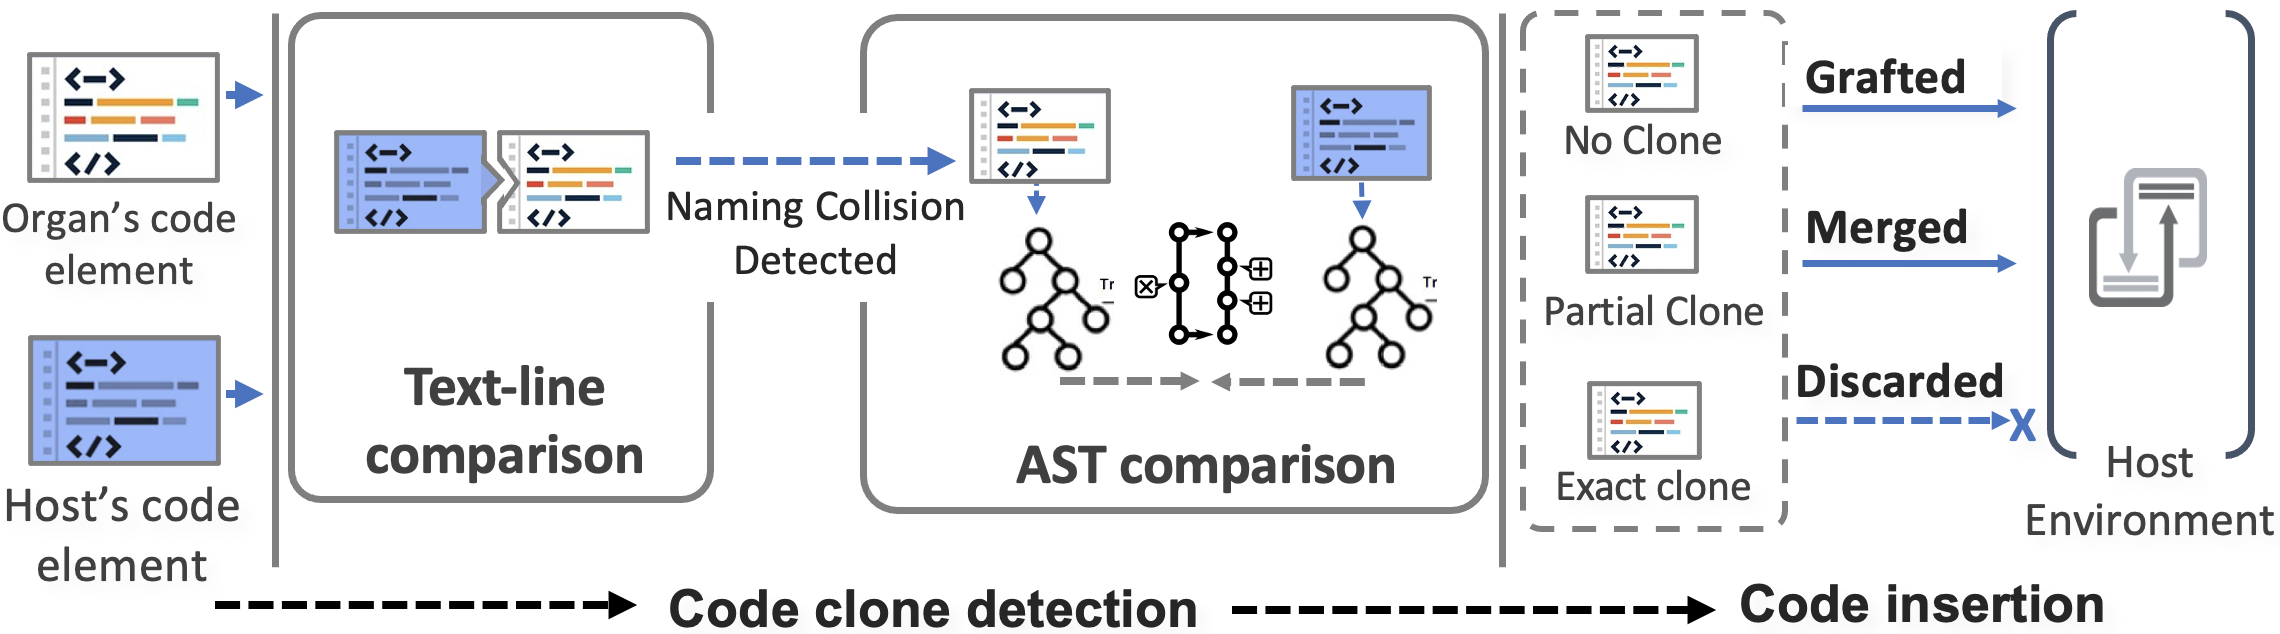
\includegraphics[width=\textwidth]{images/clone_detector.png}
	\caption{Code clone detector. \textit{It performs two comparison steps: text-line and ASTs comparisons to identify code clones and make decision if a code elements must be graft our not into the target product base environment.}}
	\label{fig:code_clone_analysis}
\end{figure} 

We augmented \prodscalpel with a \emph{code clone detector}, based on NiCad~\cite{Roy2009}. This clone detector finds exact clones over arbitrary program fragments in the organ and host source code by using ASTs. Thus, we exploit the benefits of \emph{Program differencing}~\cite{Kernighan1983} technique and TXL~\cite{Cordy2006} to identify and compare potential syntactic code duplication using text-line and ASTs comparison~\cite{Roy2009}.
